\clearpage
\section{Iteration 3 -- Project Leader and Task Ownership}

\noindent\textbf{Project leader:} \GK{} (\DS{} led Iteration 2).

\begin{table}[h]
\centering
\small
\begin{tabular}{>{\raggedright\arraybackslash}p{0.45\textwidth}ll}
\toprule
Item & Owner & Checker\\
\midrule
Small worked example, Q1, Q3 (\texttt{small\_example.py}) & \DS & \GK\\
Gaussian elimination, Q-learning (\texttt{my\_gauss\_solve}, \texttt{my\_q\_learning}), Q4 & \DS & \GK\\
MDP construction, value iteration, Q2 & \GK & \DS\\
Simulation test (\texttt{simulate.py}, \texttt{check\_simulation.py}) & \GK & \DS\\
Real data: cleaning, parser, library comparison (\texttt{run\_real.py}) & \GK & \DS\\
Q5 and assumption checks & \DS & \GK\\
Verification table, README, Excel plan & \GK & \DS\\
\bottomrule
\end{tabular}
\caption{Iteration 3 owner and checker of each item.}
\end{table}

\section{Small Worked Example}\label{sec:small}

Script: \texttt{src/small\_example.py}. Values are exact fractions except in value iteration and Q-learning.

\noindent\textbf{Maze.} A $3\times3$ maze in the competition file format, start in the bottom-left corner, goal in the centre (open only to the east). The parser (Algorithm~1, step~1) gives
\[
M = \begin{pmatrix}9&5&3\\10&13&2\\12&5&6\end{pmatrix},\qquad \text{start } s = 6,\quad \Gset = \{4\},\quad n = 9,
\]
with $s = 3r+c$, $p = \tfrac1{10}$, $\gamma = \tfrac9{10}$, $R(s) = -1$, $R(4) = 10$.

\noindent\textbf{Step 1: transition matrices} (Algorithm~1, step~2; definition of $P_a$ in Q1 of Iteration 2). Row 6 of $P_1$ (move right from the start) is $(0,0,0,\tfrac1{10},0,0,\tfrac1{10},\tfrac45,0)$: right succeeds with $\tfrac45$, the slip up reaches cell 3, the slip down hits the border and stays in cell 6.

\noindent\textbf{Step 2: rows sum to 1} (Q3). Every row of every $P_a$ sums to exactly 1.

\noindent\textbf{Step 3: fixed policy and $P_\pi$} (Algorithm~3, steps 1--2).
$\pi = \left(\begin{smallmatrix}\rightarrow&\rightarrow&\downarrow\\ \uparrow&G&\leftarrow\\ \rightarrow&\rightarrow&\uparrow\end{smallmatrix}\right)$, and row $s$ of $P_\pi$ is row $s$ of $P_{\pi(s)}$:
{\small
\[
A = I-\gamma P_\pi =
\begin{pmatrix}
\frac{91}{100}&-\frac{18}{25}&0&-\frac9{100}&0&0&0&0&0\\
0&\frac{41}{50}&-\frac{18}{25}&0&0&0&0&0&0\\
0&-\frac9{100}&\frac{91}{100}&0&0&-\frac{18}{25}&0&0&0\\
-\frac{18}{25}&0&0&\frac{41}{50}&0&0&0&0&0\\
0&0&0&0&\frac1{10}&0&0&0&0\\
0&0&-\frac9{100}&0&-\frac{18}{25}&1&0&0&-\frac9{100}\\
0&0&0&-\frac9{100}&0&0&\frac{91}{100}&-\frac{18}{25}&0\\
0&0&0&0&0&0&0&\frac{41}{50}&-\frac{18}{25}\\
0&0&0&0&0&-\frac{18}{25}&0&-\frac9{100}&\frac{91}{100}
\end{pmatrix}.
\]}

\noindent\textbf{Step 4: Gaussian elimination on $[A\mid R]$} (Algorithm~3, steps 3--4; Theorem~\ref{thm:bellman}). Column 1 needs $R_4\leftarrow R_4-(-\tfrac{72}{91})R_1$, which gives row 4 $=(0,-\tfrac{1296}{2275},0,\tfrac{3407}{4550},0,0,0,0,0\mid-\tfrac{163}{91})$. Column 2 needs $R_3\leftarrow R_3-(-\tfrac9{82})R_2$ and $R_4\leftarrow R_4-(-\tfrac{2592}{3731})R_2$. The script prints every operation and the matrix after each one. No row swap is needed. Back substitution gives
\begin{gather*}
V(0) = V(6) = \tfrac{12700809950}{244932637},\quad V(1) = V(7) = \tfrac{4413250}{71891},\quad V(2) = V(8) = \tfrac{5126050}{71891},\\
V(3) = \tfrac{10853232350}{244932637},\quad V(4) = 100,\quad V(5) = \tfrac{6026950}{71891},\\
V^\pi \approx(51.854,\ 61.388,\ 71.303,\ 44.311,\ 100,\ 83.835,\ 51.854,\ 61.388,\ 71.303).
\end{gather*}
The top and bottom rows match because the maze is symmetric about the middle row.

\noindent\textbf{Second-way check.} Substituting back gives $(I-\gamma P_\pi)V^\pi-R = 0$ exactly, and $V(4) = 100 = R(g)/(1-\gamma)$ (Proposition~\ref{prop:goal}). \texttt{numpy.linalg.solve} agrees to $2.8\times10^{-14}$.

\noindent\textbf{Step 5: value iteration} (Algorithm~2, Theorem~\ref{thm:contraction}), $V_0 = 0$. The script prints $V_k$ after each of the 242 steps; the first ones are
\begin{center}
\small
\begin{tabular}{rrrrrrrrrr}
\toprule
$k$ & $V_k(0)$ & $V_k(1)$ & $V_k(2)$ & $V_k(3)$ & $V_k(4)$ & $V_k(5)$ & $V_k(6)$ & $V_k(7)$ & $V_k(8)$\\
\midrule
1 & $-1$ & $-1$ & $-1$ & $-1$ & 10 & $-1$ & $-1$ & $-1$ & $-1$\\
2 & $-1.9$ & $-1.9$ & $-1.9$ & $-1.9$ & 19 & 6.02 & $-1.9$ & $-1.9$ & $-1.9$\\
3 & $-2.71$ & $-2.71$ & 2.992 & $-2.71$ & 27.1 & 12.338 & $-2.71$ & $-2.71$ & 2.992\\
\bottomrule
\end{tabular}
\end{center}
The reward spreads one cell per step from the goal. Every ratio $\norm{V_{k+1}-V_k}/\norm{V_k-V_{k-1}}$ is at most $0.9 = \gamma$ (largest $0.90000002$, rounding), so the error shrinks at least like $\gamma^k$. The final $V$ agrees with $V^\pi$ to $8.5\times10^{-10}$, because the fixed policy is optimal here.

\noindent\textbf{Step 6: Q-learning} (Algorithm~4): $\max_s|\max_aQ(a,s)-V^*(s)| = 1.410,\ 0.556,\ 0.211$ after $10^3, 10^4, 10^5$ episodes.

\section{From-Scratch Implementation}

All method code is in \texttt{src/methods.py}, uses NumPy arrays and products only, and runs the small example, the simulation and the real mazes. \texttt{numpy.linalg} is only used to check.

\begin{center}
\small
\begin{tabular}{>{\raggedright\arraybackslash}p{0.2\textwidth}>{\raggedright\arraybackslash}p{0.4\textwidth}>{\raggedright\arraybackslash}p{0.3\textwidth}}
\toprule
Step & Equation & Function\\
\midrule
Alg.~1.1 & $M$, start, $\Gset$; $\mathrm{next}(s,b)$ & \texttt{parse\_maze}, \texttt{my\_next\_state\_table}\\
Alg.~1.2 & $(P_a)_{s,\mathrm{next}(s,b)} \mathrel{+}= \Pr(b\mid a)$ & \texttt{my\_transition\_matrices}\\
Alg.~1.3 & $R(s) = -1$, $R(g) = 10$ & \texttt{my\_rewards}\\
Alg.~2.1 & $Q_k(a,s) = R(s)+\gamma(P_aV_k)(s)$ & \texttt{my\_bellman\_Q}\\
Alg.~2.2--2.4 & $V_{k+1} = \max_aQ_k$, stop rule, greedy $\pi$ & \texttt{my\_value\_iteration}\\
Alg.~3.1 & $(P_\pi)_{s,:} = (P_{\pi(s)})_{s,:}$ & \texttt{my\_policy\_matrix}\\
Alg.~3.3--3.4 & elimination of $[A\mid R]$, back substitution & \texttt{my\_gauss\_solve}\\
Alg.~4 & $Q(a,s)\leftarrow Q(a,s)+N(s,a)^{-0.6}(x-Q(a,s))$ & \texttt{my\_q\_learning}\\
Q5 & steps to $\Gset$ following $\pi$ & \texttt{my\_steps\_to\_goal}\\
\bottomrule
\end{tabular}
\end{center}

\noindent Two small changes since Iteration 2, both to match the starter code: $Q$ is stored as a $4\times n$ array (action first, like $P_a$), and Q-learning episodes start in a random non-goal state, so that every state the starter code compares is visited (A9).

\section{Simulation Test}

Script: \texttt{src/check\_simulation.py}. Same model, parameters and seed as Iteration 2 ($5\times5$, $p = 0.1$, $\gamma = 0.95$, seed 0), now built by \texttt{build\_maze\_mdp} in \texttt{src/simulate.py}. The true values are $V^*$; the sample size is the number of Q-learning episodes.

\noindent\textbf{With the library.} Our Gaussian elimination agrees with \texttt{numpy.linalg.solve} to $5.7\times10^{-14}$. This is rounding: both solve the same system, $\mathrm{cond}(I-\gamma P_\pi) = 145$, and machine precision is $1.1\times10^{-16}$.

\noindent\textbf{With the truth.} Value iteration agrees with the exact solution to $1.9\times10^{-9}$. This comes from the stopping rule, not rounding: by Theorem~\ref{thm:contraction}, $\norm{V_k-V^*}\le\frac{\gamma}{1-\gamma}\norm{V_k-V_{k-1}}<19\times10^{-10}$. The largest ratio of successive steps is $0.95000003\le\gamma+10^{-6}$. Q-learning: $\max_s|\max_aQ-V^*| = 26.9,\ 1.99,\ 0.55$ after 500, 5000, 50000 episodes (log--log slope $-0.85$, Figure~\ref{fig:q}). The greedy action is optimal in 24 of 25 cells; the exception is cell $(2,0)$, where right and down differ by only $0.61$ in $Q^*$. From $(0,0)$ the learned policy needs 10.2 steps on average, value iteration 10.0. The starter line prints $1.01$ and $0.96$ for 20000 episodes.

\noindent\textbf{Stress test} ($\gamma$ close to 1, A4). Value iteration needs 495 steps for $\gamma = 0.95$ and 25348 for $\gamma = 0.999$, close to the predicted $\log(10^{-10}/\norm{V_1-V_0})/\log\gamma = 494$ and $25316$.

\begin{figure}[h]
\centering
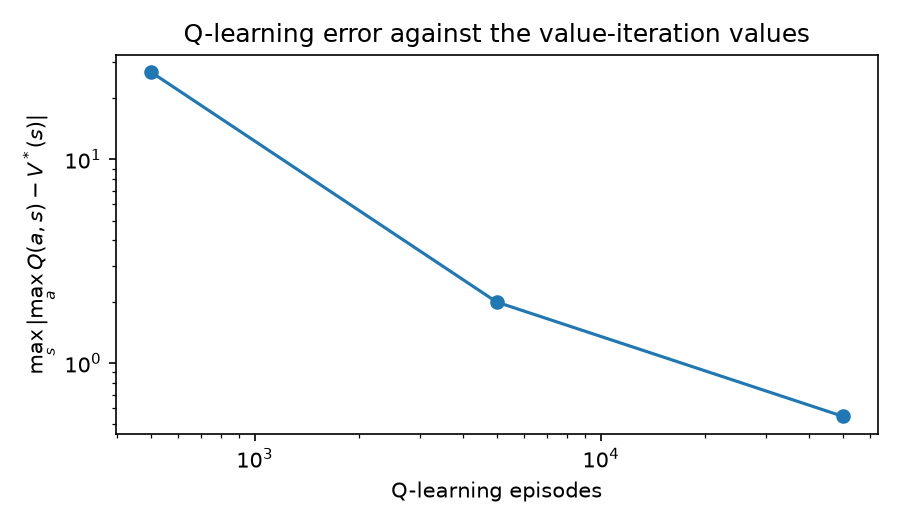
\includegraphics[width=0.55\textwidth]{figures/qlearning_error.png}
\caption{Simulation: Q-learning error against the value-iteration values.}
\label{fig:q}
\end{figure}

\section{Real Data}

Script: \texttt{src/run\_real.py}. Same $p$, $\gamma$ and rewards; $n = 256$.

\noindent\textbf{Cleaning.} 525 files. Removed: 2 files whose goal cannot be reached (\texttt{001.txt}, \texttt{001-anomaly-test.txt}, A7); 4 synthetic test layouts (\texttt{empty}, \texttt{long}, \texttt{wiggly1}, \texttt{zigzag}); 13 exact duplicates of another contest's maze (for example \texttt{AAMC17} = \texttt{AAMC16}), so that the test maze cannot also be a training maze. That leaves 506 mazes: \texttt{AAMC24Maze.txt} is kept unseen for Q5 and the other 505 are training mazes. Figure~\ref{fig:parsed} draws the parsed test maze.

\noindent\textbf{Library comparison on all 506 mazes.} Rows of every $P_a$ sum to 1 exactly. Value iteration against our Gaussian elimination: at most $1.9\times10^{-9}$ (the stopping-rule bound above). Our Gaussian elimination against \texttt{numpy.linalg.solve}: at most $6.8\times10^{-13}$ (rounding). $V^\pi$ is the unique solution of a linear system (Theorem~\ref{thm:inv}), so there is no sign or scaling convention to fix.

\begin{figure}[h]
\centering
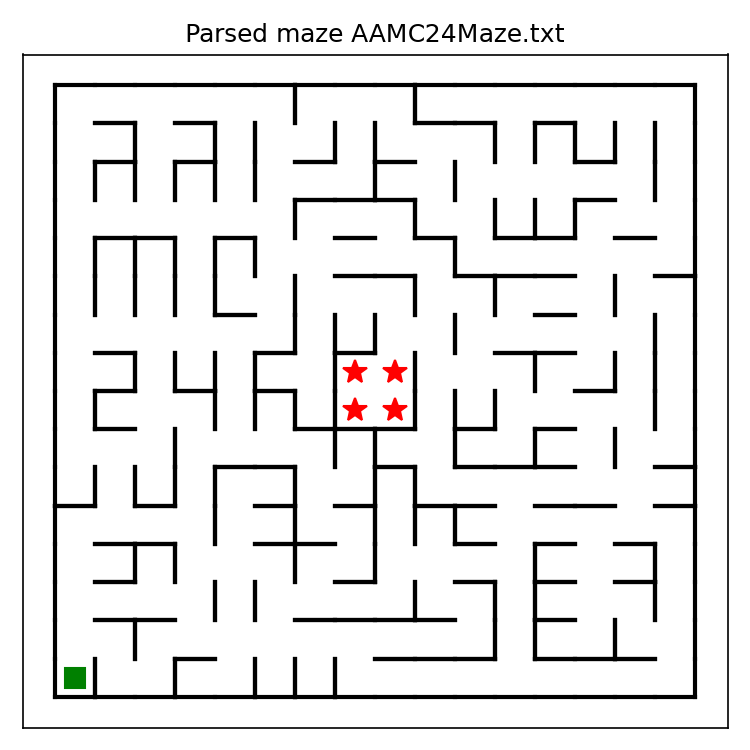
\includegraphics[width=0.35\textwidth]{figures/parsed_maze.png}
\caption{The parsed maze \texttt{AAMC24Maze.txt} (start green, goal red).}
\label{fig:parsed}
\end{figure}

\section{Verification Table}

\begin{center}
\small
\begin{tabular}{llllc}
\toprule
Data & Quantity & Compared with & Difference & Pass?\\
\midrule
Small example & $P_a\one$ & $\one$ (fractions) & 0 & \checkmark\\
Small example & $(I-\gamma P_\pi)V^\pi-R$ & 0 (fractions) & 0 & \checkmark\\
Small example & $V^\pi$ & \texttt{numpy.linalg.solve} & $\max|\cdot| = 2.8\times10^{-14}$ & \checkmark\\
Small example & $V$ (value iteration) & $V^\pi$ (fractions) & $\max|\cdot| = 8.5\times10^{-10}$ & \checkmark\\
Simulation & $V$ (value iteration) & $V$ (Gauss) & $\max|\cdot| = 1.9\times10^{-9}$ & \checkmark\\
Simulation & $V$ (Gauss) & \texttt{numpy.linalg.solve} & $\max|\cdot| = 5.7\times10^{-14}$ & \checkmark\\
Simulation & error ratio & $\gamma = 0.95$ & max $0.95000003$ & \checkmark\\
Simulation (50000 ep.) & $\max_aQ$ & $V^*$ & $\max|\cdot| = 0.55$ & \checkmark\\
Simulation (stress) & VI steps, $\gamma = 0.999$ & steps, $\gamma = 0.95$ & 25348 vs 495 & \checkmark\\
Real, 506 mazes & $P_a\one$ & $\one$ & 0 & \checkmark\\
Real, 506 mazes & $V$ (value iteration) & $V$ (Gauss) & $\max|\cdot| = 1.9\times10^{-9}$ & \checkmark\\
Real, 506 mazes & $V$ (Gauss) & \texttt{numpy.linalg.solve} & $\max|\cdot| = 6.8\times10^{-13}$ & \checkmark\\
Real, \texttt{AAMC24} & Q-learning steps & value iteration steps & 30.9 vs 30.8 & \checkmark\\
\bottomrule
\end{tabular}
\end{center}

\section{Assumption Checks}

Each check is printed by \texttt{check\_simulation.py} (simulation) and \texttt{run\_real.py} (real data).
\begin{itemize}[nosep]
\item \textbf{A1 Markov} and \textbf{A2 stationarity}: hold by construction in both, since the next cell is drawn from $(P_a)_{s,:}$ and the maze and $p$ are fixed. On an unseen maze the mouse that does not know the walls would need the walls seen so far in its state; in Q5 the mouse learns one fixed maze by repeated runs, so the cell is the state.
\item \textbf{A3}: $\max|P_a\one-\one| = 0$ in the simulation and on all 506 mazes.
\item \textbf{A4}: $\min|\lambda(I-\gamma P_\pi)| = 0.05 = 1-\gamma$ in both; $\mathrm{cond}(I-\gamma P_\pi) = 145$ (simulation) and $297$ (\texttt{AAMC24}). The stress test shows the cost of $\gamma$ near 1.
\item \textbf{A5}: $\max|R| = 10$. \textbf{A6}: 25 and 256 states, 4 actions.
\item \textbf{A7}: in the simulation the optimal policy reaches the goal from $(0,0)$ in all 200 runs (at most 17 steps); 2 real files removed.
\item \textbf{A8}: by design, \texttt{my\_q\_learning} only uses sampled moves.
\item \textbf{A9}: minimum visits $N(s,a)$ over non-goal states: 27 (simulation, 20000 episodes) and 17 over reachable cells (\texttt{AAMC24}, 30000 episodes).
\end{itemize}

\section{Iteration 3 -- Math Questions}

\noindent\textbf{Q1.} Section~\ref{sec:small}, steps 1--4: $V^\pi\approx(51.854, 61.388, 71.303, 44.311, 100,$ $83.835, 51.854, 61.388, 71.303)$ in exact fractions; \texttt{numpy.linalg.solve} agrees to $2.8\times10^{-14}$.
\signoff{\DS}{\GK}

\noindent\textbf{Q2.} Section~\ref{sec:small}, step 5: $V_k$ is printed at all 242 steps, and every ratio of successive errors is at most $\gamma = 0.9$, so $\norm{V_k-V_{k-1}}\le\gamma^{k-1}\norm{V_1-V_0}$. In the simulation the largest ratio is $0.95000003$.
\signoff{\GK}{\DS}

\noindent\textbf{Q3.} Every row sums to exactly 1 in the small example, the simulation and all 506 real mazes, because row $s$ of $P_a$ adds $(1-2p)+p+p = 1$.
\signoff{\DS}{\GK}

\noindent\textbf{Q4.} On the small maze the Q-learning error falls from 1.410 to 0.556 to 0.211 for $10^3$, $10^4$, $10^5$ episodes; in the simulation from 26.9 to 0.55 for 500 to 50000 episodes.
\signoff{\DS}{\GK}

\noindent\textbf{Q5.} A Q-table belongs to one maze, so we train Q-learning (Algorithm~4, 30000 episodes) on each maze. On 10 random training mazes the greedy route reaches the goal on the 7 mazes whose shortest path is at most 51 cells, within 10\% of the value-iteration policy (the largest gap is 47.8 vs 43.8 steps on \texttt{AAMC18}), and never reaches the goal on the 3 with paths of 65, 77 and 86 cells: there, 30000 episodes of at most 200 steps do not carry the goal reward back to the start. On the unseen maze \texttt{AAMC24} (shortest path 22 cells) the trained mouse needs 30.9 steps on average, against 30.8 for the value-iteration policy.
\signoff{\DS}{\GK}
